% f1_overview.tex -- Figure 1 (in the title block): the three steps of the method in one row (natural width about 17.4 cm).
%   Colours: navy = in-distribution side, grey = re-oriented images, red = what is computed for the test image and the point mu*.
%   Panels 2 and 3 are schematics (the drawing to scale is Figure 4; there mu* is 8 times as far from mu as mu_o).
\begin{tikzpicture}[>={Stealth[length=2mm, width=1.6mm]}, font=\footnotesize, line cap=round, line join=round,
  ttl/.style={anchor=north west, inner sep=0pt, font=\small}, lab/.style={font=\footnotesize, inner sep=1pt, align=center},
  sm/.style={font=\scriptsize, inner sep=1pt, align=center}]
% frames of the three steps (no fill)
\draw[black!40, rounded corners=4pt] (0,0) rectangle (5.5,3.9);
\draw[black!40, rounded corners=4pt] (5.95,0) rectangle (11.45,3.9);
\draw[black!40, rounded corners=4pt] (11.9,0) rectangle (17.4,3.9);
\draw[->, very thick] (5.55,1.9) -- (5.9,1.9);
\draw[->, very thick] (11.5,1.9) -- (11.85,1.9);
% ---------------------------------------------------------------- 1
\node[ttl] at (0.15,3.75) {\textbf{1.}\ 画像1枚から数を $p$ 個とる};
\node[inner sep=0, draw=black!50, line width=0.4pt] (im) at (0.75,1.85) {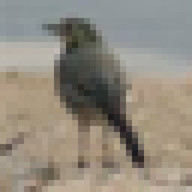
\includegraphics[width=1.05cm]{img/b_o0.png}};
\node[lab, anchor=north] at (0.75,1.27) {画像 $\vec{x}$};
\draw[->] (1.35,1.85) -- (1.75,1.85);
\begin{scope}[shift={(1.85,1.85)}]
  \foreach \dx/\yc/\h in {0/0.1/1.3, 0.22/0.1/1.3, 0.44/-0.1/0.9, 0.66/-0.1/0.9, 0.88/-0.25/0.6, 1.1/-0.25/0.6}
    \draw[black, line width=0.45pt] (\dx,\yc-\h/2) rectangle ++(0.13,\h);
  \draw[redc, line width=1.0pt] (1.32,-0.1-0.45) rectangle ++(0.13,0.9);
  \foreach \dx/\yc/\h in {1.54/-0.1/0.9, 1.76/0.1/1.3, 1.98/0.1/1.3}
    \draw[black!35, densely dashed, line width=0.4pt] (\dx,\yc-\h/2) rectangle ++(0.13,\h);
\end{scope}
\node[lab] at (2.9,2.98) {U-Net(凍結)};
\node[lab, text=redc] at (3.23,0.95) {A で止める};
\draw[->] (4.0,1.85) -- (4.4,1.85);
\begin{scope}[shift={(4.55,2.65)}]
  \foreach \k/\t in {0/{a_{1}}, 1/{a_{2}}} \draw[line width=0.45pt] (0,{-0.36*\k}) rectangle ++(0.5,-0.36) node[midway, sm] {$\t$};
  \node[sm] at (0.25,-0.92) {$\vdots$};
  \draw[line width=0.45pt] (0,-1.2) rectangle ++(0.5,-0.36) node[midway, sm] {$a_{p}$};
  \node[sm, anchor=south] at (0.25,0.03) {$\vec{a}(\vec{x})$};
  \node[sm, anchor=north] at (0.25,-1.6) {$p{\times}1$};
\end{scope}
\node[sm, anchor=south] at (2.75,0.12) {ブロックごとに数を1つ};
% ---------------------------------------------------------------- 2
\node[ttl] at (6.1,3.75) {\textbf{2.}\ 基準点 $\vec{\mu}^{*}$ を決める(事前に1回)};
\draw[black!50, line width=0.6pt, rotate around={25:(7.1,1.05)}] (7.1,1.05) ellipse (0.75 and 0.36);
\fill[black!60] (7.1,1.05) circle (1.7pt);
\node[sm, text=black!65, anchor=north] at (7.25,0.6) {向きを変えた画像};
\node[sm, anchor=north west] at (7.12,1.0) {$\vec{\mu}_{o}$};
\draw[navyc, line width=0.9pt, rotate around={25:(8.55,1.72)}] (8.55,1.72) ellipse (0.75 and 0.36);
\fill[navyc] (8.55,1.72) circle (1.8pt);
\node[sm, text=navyc, anchor=north west] at (8.62,1.67) {$\vec{\mu}$};
\node[sm, text=navyc, anchor=north west] at (9.15,1.4) {分布内の画像};
\draw[->, line width=0.8pt] (7.17,1.08) -- (8.47,1.68);
\node[sm, anchor=south east] at (7.85,1.42) {$\vec{\mu}-\vec{\mu}_{o}$};
\draw[redc, densely dashed, line width=0.8pt] (8.63,1.76) -- (9.55,2.19);
\draw[redc, line width=0.6pt] (9.52,2.32) -- (9.62,2.06) (9.62,2.37) -- (9.72,2.11);
\draw[->, redc, densely dashed, line width=0.8pt] (9.68,2.25) -- (10.6,2.68);
\node[redc, font=\large, inner sep=0] at (10.7,2.73) {$\star$};
\node[sm, text=redc, anchor=south east] at (10.65,2.8) {$\vec{\mu}^{*}$};
\node[sm, text=redc, anchor=south east, align=right] at (9.5,2.3) {$c(\vec{\mu}-\vec{\mu}_{o})$\\$c=8$};
% ---------------------------------------------------------------- 3
\node[ttl] at (12.05,3.75) {\textbf{3.}\ テスト画像のスコア};
\begin{scope}
  \clip (11.95,0.05) rectangle (17.35,3.3);
  \foreach \s in {1,1.9,2.8}
    \draw[redc!70, densely dashed, line width=0.5pt, rotate around={25:(16.0,2.3)}] (16.0,2.3) ellipse ({0.75*\s} and {0.36*\s});
\end{scope}
\node[redc, font=\large, inner sep=0] at (16.0,2.3) {$\star$};
\node[sm, text=redc, anchor=west, fill=white, inner sep=0.5pt] at (16.15,2.3) {$\vec{\mu}^{*}$};
\fill[redc] (12.75,1.1) circle (2pt);
\node[sm, text=redc, anchor=north, fill=white, inner sep=1pt] at (12.8,1.0) {テスト画像};
\draw[redc, line width=0.8pt] (12.8,1.12) -- (15.9,2.26);
\node[sm, text=redc, rotate=20, anchor=south, fill=white, inner sep=0.5pt] at (14.3,1.7) {距離};
\node[sm, anchor=south east, align=right, fill=white, inner sep=1pt] at (17.3,0.12) {スコア $s(\vec{x})$ は数1つ\\近いほど分布内らしい};
\end{tikzpicture}
